\documentclass{beamer}
\usepackage[utf8]{inputenc}

\usetheme{Madrid}
\usecolortheme{default}
\usepackage{amsmath,amssymb,amsfonts,amsthm}
\usepackage{txfonts}
\usepackage{tkz-euclide}
\usepackage{listings}
\usepackage{adjustbox}
\usepackage{array}
\usepackage{tabularx}
\usepackage{gvv}
\usepackage{lmodern}
\usepackage{circuitikz}
\usepackage{tikz}
\usepackage{graphicx}

\setbeamertemplate{page number in head/foot}[totalframenumber]

\usepackage{tcolorbox}
\tcbuselibrary{minted,breakable,xparse,skins}



\definecolor{bg}{gray}{0.95}
\DeclareTCBListing{mintedbox}{O{}m!O{}}{%
  breakable=true,
  listing engine=minted,
  listing only,
  minted language=#2,
  minted style=default,
  minted options={%
    linenos,
    gobble=0,
    breaklines=true,
    breakafter=,,
    fontsize=\small,
    numbersep=8pt,
    #1},
  boxsep=0pt,
  left skip=0pt,
  right skip=0pt,
  left=25pt,
  right=0pt,
  top=3pt,
  bottom=3pt,
  arc=5pt,
  leftrule=0pt,
  rightrule=0pt,
  bottomrule=2pt,
  toprule=2pt,
  colback=bg,
  colframe=orange!70,
  enhanced,
  overlay={%
    \begin{tcbclipinterior}
    \fill[orange!20!white] (frame.south west) rectangle ([xshift=20pt]frame.north west);
    \end{tcbclipinterior}},
  #3,
}
\lstset{
    language=C,
    basicstyle=\ttfamily\small,
    keywordstyle=\color{blue},
    stringstyle=\color{orange},
    commentstyle=\color{green!60!black},
    numbers=left,
    numberstyle=\tiny\color{gray},
    breaklines=true,
    showstringspaces=false,
}
%------------------------------------------------------------
%This block of code defines the information to appear in the
%Title page
\title %optional
{1.9.16}
\date{Agust, 2025}
%\subtitle{A short story}

\author % (optional)
{INDHIRESH S - EE25BTECH11027}



\begin{document}


\frame{\titlepage}
\begin{frame}{Question}
Find the distance between the points $(a, b)$ and $(-a, -b)$.
\end{frame}
\begin{frame}{allowframebreaks}
\frametitle{Equation}

    \centering
    
    \label{tab:parameters}
  Let the given two points be P and Q, where,
\begin{align}
    \Vec{P}=\myvec{a\\b} \; and\; \Vec{Q}=\myvec{-a\\-b}
\end{align}
	Let \Vec{D} be a vector defined as:
\begin{align}
	\Vec{D}=\Vec{P}-\Vec{Q}   
\end{align}
   
\end{frame}


\begin{frame}{Theoretical Solution}
Now,
\begin{align}
	\Vec{D}=\myvec{a\\b}-\myvec{-a\\-b}
\end{align}
\begin{align}
	\Vec{D}=\myvec{2a\\2b}
\end{align}
	The distance between the point P and Q $=$ Norm of the vector D\\
	Norm of the vector D is defined as:
\begin{align}
    ||D||\triangleq\sqrt{D^TD}
\end{align}
\begin{align}
    D^TD=\myvec{2a&2b}\myvec{2a\\2b}
\end{align}
\begin{align}
    D^TD=4a^2+4b^2
\end{align}

\end{frame}
\begin{frame}
\frametitle{Theoretical Solution}
Now substituite in Eq.5:
\begin{align}
    ||D||=\sqrt{4a^2+4b^2}
\end{align}
\begin{align}
    ||D||=2\sqrt{a^2+b^2}
\end{align}
Therefore the distance between the two points is:    $2\sqrt{a^2+b^2}$\\\\
For verification let us assume $a=4\;and\; b=4$\\

\end{frame}



\begin{frame}[fragile]
    \frametitle{C Code - Midpoint formula }

    \begin{lstlisting}
#include <stdio.h>
#include <math.h>

// Function to calculate distance
float distance(float a, float b) {
    float x1 = a, y1 = b;
    float x2 = -a, y2 = -b;

    float dist = sqrt((x2 - x1)*(x2 - x1) + (y2 - y1)*(y2 - y1));
    return dist;
}



    \end{lstlisting}
\end{frame}


\begin{frame}[fragile]
    \frametitle{Python Code}
    \begin{lstlisting}
import numpy as np
import ctypes
import matplotlib.pyplot as plt

# Load the shared library
lib = ctypes.CDLL("./midpoint.so")   # use "midpoint.dll" on Windows

# Define function signature
lib.midpoint.argtypes = [
    ctypes.c_float, ctypes.c_float,  # x1, y1
    ctypes.c_float, ctypes.c_float,  # x2, y2
    ctypes.POINTER(ctypes.c_float),  # mx
    ctypes.POINTER(ctypes.c_float)   # my
]






    \end{lstlisting}
\end{frame}

\begin{frame}[fragile]
    \frametitle{Python Code}
    \begin{lstlisting}
import ctypes
import matplotlib.pyplot as plt

# Load shared C library
lib = ctypes.CDLL("./c.so")
lib.distance.argtypes = [ctypes.c_float, ctypes.c_float]
lib.distance.restype = ctypes.c_float

# Example values
a, b = 4, 4  # change as needed

# Call C function
dist = lib.distance(a, b)
print(f"Distance between ({a},{b}) and (-{a},-{b}) = {dist}")

# Coordinates
x1, y1 = a, b
x2, y2 = -a, -b







    \end{lstlisting}
\end{frame}

\begin{frame}[fragile]
    \frametitle{Python Code}

    \begin{lstlisting}
# Plot
plt.figure(figsize=(6,6))

# Line between points
plt.plot([x1, x2], [y1, y2], "b-", label=f"Distance = {dist:.2f}")

# Points
plt.scatter(x1, y1, color="red", s=100, label=f"A({x1}, {y1})")
plt.scatter(x2, y2, color="green", s=100, label=f"B({x2}, {y2})")

# Labels near points
plt.text(x1+0.2, y1, f"A({x1}, {y1})", fontsize=10, color="red")
plt.text(x2-1.5, y2, f"B({x2}, {y2})", fontsize=10, color="green")



    \end{lstlisting}
\end{frame}
\begin{frame}[fragile]
    \frametitle{Python Code}

    \begin{lstlisting}
# Axes + Grid
plt.axhline(0, color="black", linewidth=0.7)
plt.axvline(0, color="black", linewidth=0.7)
plt.xlabel("X-axis")
plt.ylabel("Y-axis")
plt.title("Distance using C + Python")
plt.grid(True)
plt.legend()
plt.show()


    \end{lstlisting}
\end{frame}



\begin{frame}{Plot}
    \begin{center}
        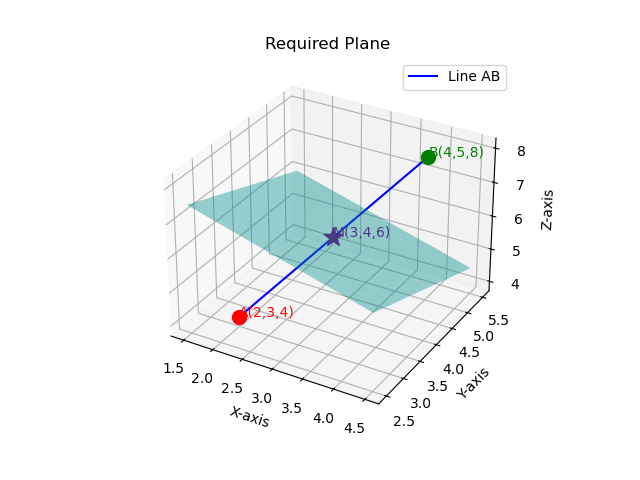
\includegraphics[width=\columnwidth, height=0.8\textheight, keepaspectratio]{figs/figure1.png}
    \end{center}
\end{frame}




\end{document}
